\section*{Informations générales}
 
\begin{table}[h]
\centering
	\begin{tabularx}{16.8cm}{|X|X|}
	\hline
	\rowcolor{gray!40} Numéro du risque & Type du risque \\
	\hline
	010 & Problème avec la CNIL\\
	\hline
	\end{tabularx}
\end{table}

\begin{table}[h]
\centering
	\begin{tabularx}{12.8cm}{|X|X|X|}
	\hline
	\rowcolor{gray!40} Date & Visa du \RQ & Visa du \CP \\
	\hline
	 27/01/16 & pgpic & pgpic \\
	\hline
	\end{tabularx}
\end{table}

\begin{table}[h]
\centering
	\begin{tabularx}{12.8cm}{|X|X|X|X|}
	\hline
	\rowcolor{gray!40} Pilote & Activité WBS & Compte WBS & Phase d'apparition \\
	\hline
	 \Pierre & Suivre les Risques et Opportunités & 1.2.3.2 & À partir du remplissage de la BD \\
	\hline
	\end{tabularx}
\end{table}

\section*{Description du risque}

\subsection*{Résumé}
	Le risque lié à un problème avec la CNIL peut entraîner des problèmes d'ordre juridique pouvant stopper brutalement le projet.
	
\subsection*{Analyse des causes}
	voir figure.

\subsection*{Criticité}

\begin{table}[h]
\centering
	\begin{tabularx}{12.8cm}{|>{}X|X|}
	\hline
	Gravité & 3\\
	\hline
	Probabilité & 2\\
	\hline
	Criticité & A surveiller\\
	\hline
	\end{tabularx}
\end{table}
\newpage

\section*{Actions}
\subsection*{Actions préventives}

%\begin{table}[H]
\centering
	\begin{longtable}{|p{7cm}|p{7cm}|}
	\hline
	\rowcolor{gray!40} Numéro de cause & Actions préventives \\
	\hline
	 1 & \begin{itemize}
	 	\item S'informer sur la législation en vigueur.
	 \end{itemize} \\
	\hline

	\end{longtable}
%\end{table}

\flushleft
\subsection*{Plan de contournement}

\begin{enumerate}
	\item Déterminer les cause de l'alerte de la CNIL
	\item Prévenir le client ainsi que le tuteur pédagogique
	\item Revoir notre gestion des informations personnelles
	\item Elaborer un nouveau dossier pour la CNIL
\end{enumerate}

\section*{Décision de clôture}
Par le \CP{} et le pilote du risque.
\begin{table}[H]
\centering
	\begin{tabularx}{12.8cm}{|X|X|}
	\hline
	\rowcolor{gray!40} Date de clôture & Raison de la clôture \\
	\hline
	  & \\
	\hline
	\end{tabularx}
\end{table}

\section*{Historique des modifications}
\begin{table}[H]
\centering
	\begin{tabularx}{12.8cm}{|X|X|}
	\hline
	\rowcolor{gray!40} Date & Modification \\
	\hline
	  & \\
	\hline
	\end{tabularx}
\end{table}
\newpage


\begin{figure}
	\centering
	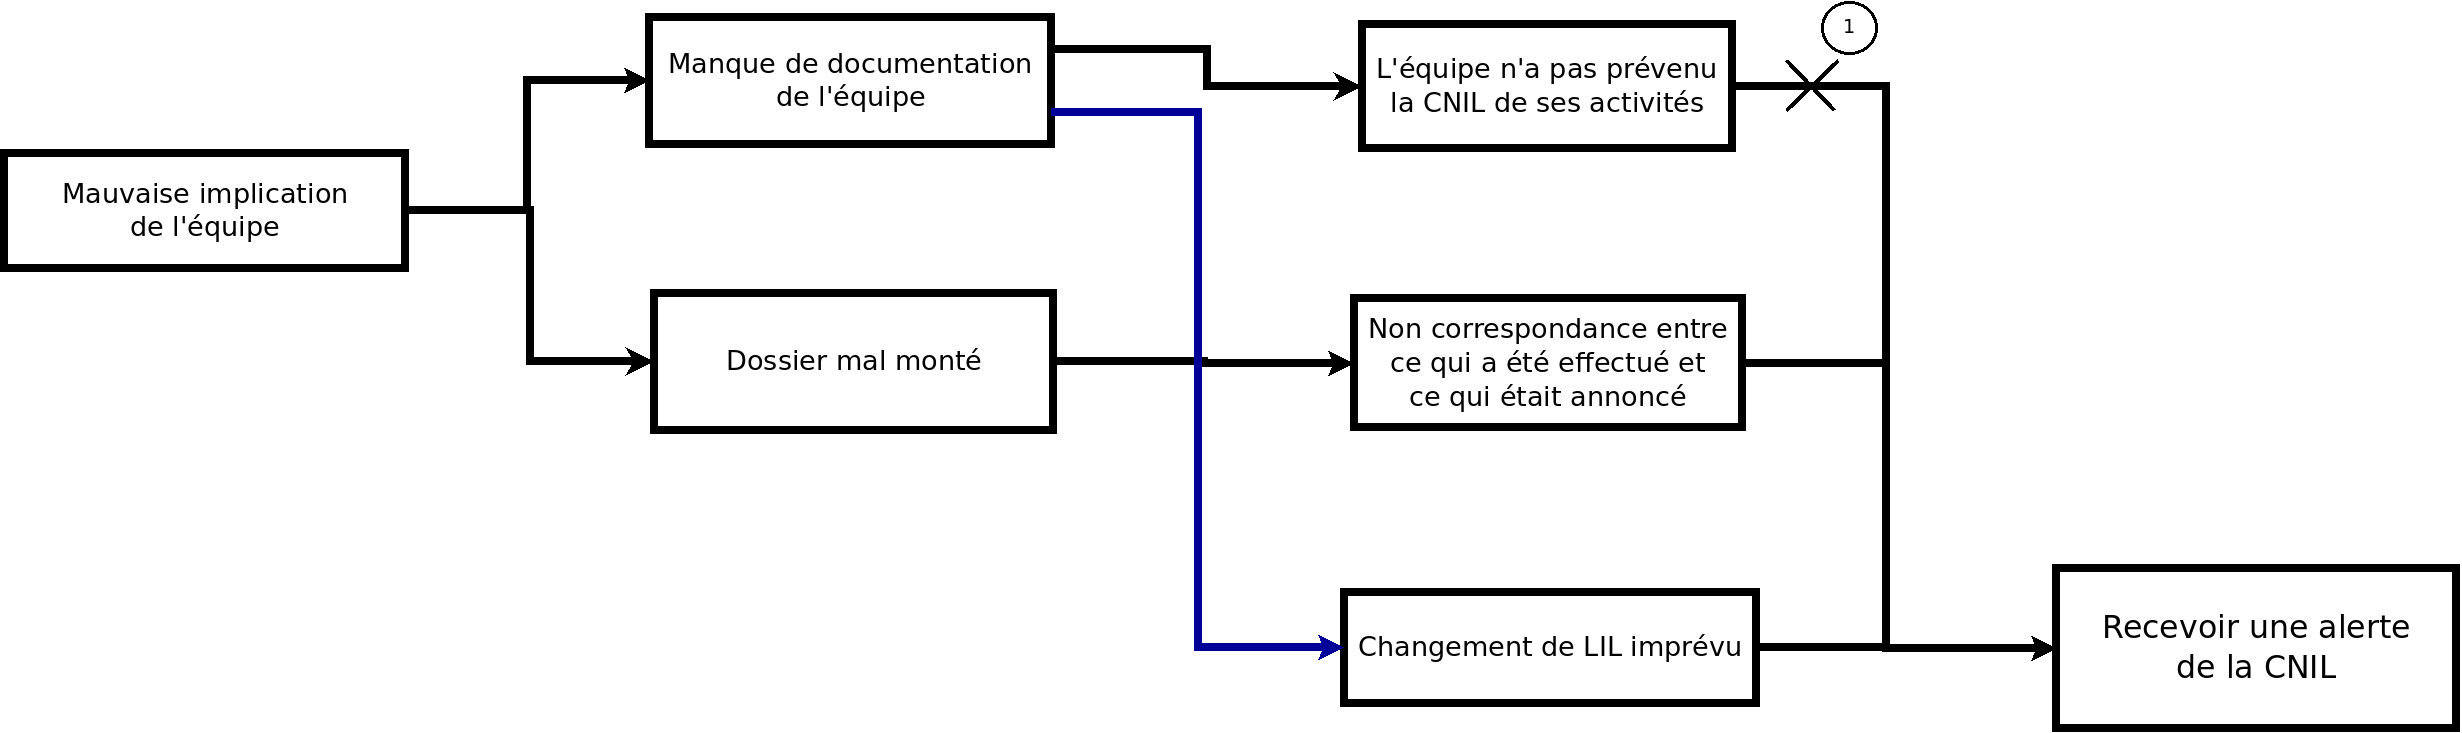
\includegraphics[scale=0.20]{images/AnalyseRisque_nPourquoi_FDR010.png}
\end{figure}